\documentclass[10pt]{article}

\usepackage[margin=1in, letterpaper]{geometry}
\usepackage{parskip}

\usepackage{amsthm, amsmath, amssymb}
% \usepackage{gensymb}  % For use of degree symbol
\usepackage[pdftex]{graphicx}
\usepackage{hyperref}

\usepackage{enumerate} % For use of (a), (b), et cetera
\usepackage{booktabs} % Tables
\usepackage[margin=20pt, labelfont=bf, labelsep=period,
justification=justified]{caption} % Captions in figure floats

% The following metadata will show up in the PDF properties
\hypersetup{
	colorlinks = true,
	urlcolor = blue,
	pdfauthor = {Aaron Tran},
	pdfkeywords = {x-ray, SNR, notes},
	pdftitle = {Supernova remnants and stuff - \today},
%	pdfsubject = {},
	pdfpagemode = UseNone
}

% Don't indent paragraphs
\setlength\parindent{0em}

% ===============
% Useful commands
% ===============
\newcommand{\mt}{\mathrm}
\newcommand{\unit}[1]{\; \mt{#1}} % vemod.net/typesetting-units-in-latex
\newcommand{\abt}{\mathord{\sim}} % tex.stackexchange.com/q/55701
\newcommand{\del}{\nabla}
\newcommand{\ptl}{\partial} % Laziness

\newcommand{\Chandra}{\textit{Chandra}}

% ===============
% Document proper
% ===============
\begin{document}

\begin{center}
    \Large{Brief review of SNR filament models of Ressler et al.}

    \normalsize{Aaron Tran}\\
    \today \\
\end{center}

\tableofcontents

% ============
% Introduction
% ============
\section{Introduction}

\subsection{Thin synchrotron rim physics}

Accelerating ISM/CSM particles in the forward shocks of supernovae emit
synchrotron radiation.  Emission is strong in the shock's immediate wake, but
dies off quickly downstream as particles radiate and lose energy. The radiation
from a spherical blast wave, then, is shell-like with bright X-ray and radio
rims/filaments due to line-of-sight projection.  These filaments have finite
and energy-dependent widths, set by:
\begin{itemize}
  \item \emph{synchrotron losses}.  At the shock, high energy electrons
  efficiently radiate harder x-ray photons.  As electrons are advected
  downstream while radiating, they radiate at lower energies and lose energy
  more slowly.  Synchrotron losses depend on (1) the initial electron energy
  distribution, and (2) the gradual decrease of electron energies downstream of
  the shock.
  \item \emph{diffusion}.  Random motion with respect to bulk plasma advection.
  Higher energy electrons diffuse and travel further downstream than would be
  expected from pure advection; hence, higher energy radiation may be seen
  farther downstream of the shock than expected.
  Higher energy particles may also diffuse \emph{ahead} of the shock, possibly
  giving rise to a so-called ``cosmic-ray shock precursor''.  Note that this is
  distinct from radiative precursors (e.g., Ghavamian et al., 2000).
\end{itemize}

\begin{figure}[!ht]
  \centering
  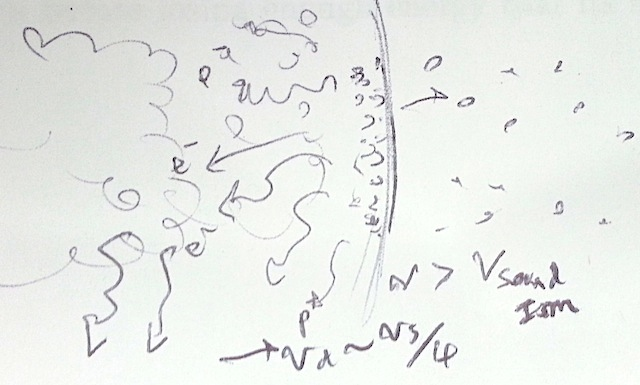
\includegraphics[scale=0.3]{doodle.jpg}
  \caption{Crude doodle of particle acceleration at a shock.
  The shock propagates into a thin, low density ISM and bounces particles
  around like crazy.  Higher energy particles diffuse randomly both behind
  and ahead of the shock.  Lower energy particles are advected \emph{backwards}
  in a reference frame co-moving with the shock. Bulk velocity, pressure, and
  density ramp down behind the shock following the Sedov-Taylor solution (?).}
  \label{fig:shock}
\end{figure}

Synchrotron losses and particle diffusion are in turn both controlled by
(1) the injected electron spectrum, and (2) the amplified magnetic field.
The amplified magnetic field may be constant, or vary in space -- e.g.
magnetic damping predicts a rapid fall off of amplification behind the shock.
Diffusion is also controlled by the nature of turbulence in the shocked plasma,
quantified by a turbulent energy/wavenumber spectrum or similar.

Synchrotron losses cause the rims to \emph{thin} with increasing energy, with
higher energy emission closer to the shock front; the characteristic length
scale falls off with radiation frequency as $l \propto \nu^{-1/2}$.  Diffusion
weakens this energy dependence, as the rims smear out more at higher energies.

\subsection{What can be said}

The width-energy dependence of synchrotron rims, and their absolute widths,
is determined by the ambient conditions (magnetic field amplification, plasma
turbulence) that control particle acceleration and diffusion.  By measuring the
energy scaling, we deduce properties of particle diffusion; by measuring the
absolute widths, we deduce information about magnetic field strength
and diffusion in some combination of parameters.

Sean considers several models that simultaneously constrain magnetic fields and
particle diffusion parameters from width measurements of these thin filaments.
The key measurables are:
\begin{itemize}
  \item magnetic field strength $B_0$ (and damping parameters, if relevant)
  \item diffusion coefficient constant $\eta_2$
  \item diffusion scaling $\mu$ (set by turbulent energy spectrum).
\end{itemize}

Here I retrace and explain relevant equations and fitting procedures from
Sean's paper; table, figure, and equation references are from the version of
record at \href{http://dx.doi.org/10.1088/0004-637X/790/2/85}
{doi:10.1088/0004-637X/790/2/85}.

% ============================
% Synchrotron rim width models
% ============================
\section{Filament width models -- theory}

Filament widths are determined by electron transport downstream of the forward
shock.  The 1-D transport equation for electron distribution $f(E,x)$
(where $E$ is electron energy, $x$ is radial coordinate) is:
\[
  \frac{\ptl f}{\ptl t} + \del \cdot \left( f \vec{v} \right)
  = C + \del \cdot \left( D \del f \right)
\]
where $C$ is an arbitrary sink/source term, $D$ is diffusion coefficient, and
$\vec{v}$ is bulk/advective plasma velocity.  With some simplifications
(1-D flow, neglect time-dependence, compressible flow unimportant,
space-independent diffusion coefficient), we obtain:
\[
    v \frac{\ptl f}{\ptl x} - D \frac{\ptl^2 f}{\ptl x^2} = C
\]
Here we have neglected two terms: $(2 D / r) (\ptl f /\ptl r)$ and
$f (\del\cdot\vec{v})$. Both terms are negligible provided that rim width
(characteristic lengthscale for $f$) is much smaller than remnant shock radius.

Two models, which both solve this transport equation, are fitted to rim width
measurements in Tables 7 and 8.  The models differ in choice of source/sink
terms ($C$) to describe synchrotron energy losses (in practice, the models
differ substantially in implementation as described further on).

% -------------------------
% Castrophic dump model (6)
% -------------------------
\subsection{Catastrophic dump model}

This model is described by equations (5--11) in Sean's paper, with (being
explicit about energy dependence):
\[
  C = -\frac{f(E,x)}{\tau_{\mt{synch}}(E)}\text{,}
\]
i.e., electrons dump their energy over a synchrotron cooling time and do not
decrease in energy as they are advected.

The model predicts rim widths (equation 6) with an approximate projection
factor $\beta = 4.6$; this implicitly assumes spherical symmetry and the
$\delta$-function approximation for synchrotron emissivity (Ballet, 2006).

References: Parizot et al. (2006), V\"{o}lk et al. (1981), Berezhko and
V\"{o}lk (2004), Ballet (2006).

% -------------------------------------
% continuous loss model (12), (14)-(16)
% -------------------------------------
\subsection{Continuous loss model}

This model is described by equations (12) and (14)-(16) in Sean's paper, with:
\[
  C = K_0 E^{-s} e^{-E/E_{\mt{cut}}} \delta(x) + \frac{\ptl}{\ptl E}
      \left(bB^2E^2f\right)
\]
representing an injected electron spectrum and an energy loss term.  Note that
$b B^2 E^2$ is proportional to synchrotron radiative power (Condon and Ransom,
\href{http://www.cv.nrao.edu/course/astr534/SynchrotronPower.html}{ERA}).

Equation (12) admits an integral form solution for particle distribution
(or, electron energy spectrum) $f(E,x)$ given by equations (14--17).
The single-particle synchrotron emissivity is integrated over the particle
distribution to obtain the full synchrotron emissivity $j_\nu$ of
our electron population (equation 20).  Then the emissivity is integrated over
lines of sight to obtain intensity profiles $I_\nu(r)$ (equation 21).
We obtain model predictions for filament FWHMs from these intensity profiles.

The single-particle synchrotron emissivity is tabulated in Appendix 2 of
Pacholczyk (1970).

References: Berezhko et al. (2003), Berezhko and V\"{o}lk (2004),
Cassam-Chena\"{i} et al. (2007), Morlino et al. (2010), and Rettig and Pohl
(2012).

% ===================
% Abbreviated summary
% ===================
\section{Filament width models -- fitting}

Tables 7, 8 summarize results from the two different models.  The key outputs
are $\eta_2$ and $B_0$ for various values of $\mu$; $\eta_2$ quantifies
diffusion strength while $B_0$ is magnetic field strength.
Sean argued that strong energy-dependence ruled out magnetic damping and did
not present fit results for magnetic damping models in SN 1006.

Why was $\mu$ fixed?  I speculate that it might have been necessary to make
fitting tractable / give useful output (note: \emph{non-linear} fitting with
3 points and 3 unknowns is not necessarily fully determined?).

All equations use the generalized diffusion coefficient $D \propto E^\mu$.

\subsection{Catastrophic dump model}

This is an analytic approximation; please see the relevant assumptions and
approximations above.  Equation (6), multiplied by a projection factor
$\beta=4.6$, is fit directly to measured rim widths as a function of energy.  
The predicted rim width is given by:
\[
  \mt{FWHM} = \frac{2\beta D / v_d}
              {\sqrt{1 + 4D/\left(v_d^2 \tau_{\mt{synch}}\right) } - 1}
\]
Table 7 presents fit results with errors that appear to be taken
from diagonal elements of the covariance matrix (which may not be safe for
non-linear fits -- needs to be checked).

Some remarks:
\begin{itemize}
  \item For Tycho, as we have 4-5 energy bands available, fitting three
  parameters ($\mu$, $\eta_2$, $B_0$) simultaneously may be tractable.
  \item As we fit equation (6) to measurements directly, we don't calculate
  $m_E$ anywhere.  However, the fit results specify $m_E(E)$ as equation (23).
  Equation (23) is only valid for the approximate model of equation (6).
  \item We could convolve the general synchrotron emissivity (equation 20) with
  the exponential electron spectrum $f(E,x)$, as is done for the complex model.
  But, probably not necessary (as this is already just an approximation).
\end{itemize}

The code for this model is given in {\tt{Widthfun.py}}.

\subsection{Continuous loss model}

The solution to equation (12) gives filament intensity profiles and hence FWHMs
to manually fit rim width measurements.  Given input parameters $\mu, \eta_2,
B_0$, FWHMs in each energy band are computed as follows:
\begin{enumerate}
  \item Integrate and solve for $f(E,x)$ using one of equations (14--16).
    Use equation (17) or (24) for the function $z(x)$ in equations (14--16),
    depending on whether you want a loss-limited or magnetically damped model.
    Change variables to make Green's function integrals numerically tractable.
  \item Compute synchrotron emissivity $j_\nu$ by integrating single-particle
    synchrotron emissivity $G(y)$ over particle distribution $f(E,x)$;
    $G(y)$ is tabulated in Pacholczyk (1970) (and interpolated as needed??).
  \item Compute intensity profile $I_\nu(r)$ by integrating emissivity $j_\nu$
    along lines of sight.
  \item Calculate FWHM of intensity profile.
\end{enumerate}
All integrals are evaluated numerically. This is resolution dependent
(discretizing electron energy, radial coordinate, line of sight coordinate),
but it should not matter too much.

Sean's manual fitting procedure computed the FWHM at 2 keV and the exponent
$m_E$ value at 2 keV (calculated from predicted FWHMs at 2 keV and 1 keV).
Per his guide, he chose $\eta_2$ to best fit $m_E$ value, then varied $B_0$ to
fit the FWHM (as $m_E$ is insensitive to $B_0$).  He ignored the FWHM at 0.7
keV for this procedure.  It would be ideal, per Sean's emails, to improve the
code to find best fit values for all FWHMs simultaneously.

The code for this model is given in {\tt{FullEfflength.f}}.  Sean's guide says
there is code for the magnetic damping model, but I'm not sure where it is.  My
guess is that it's buried in the functions for numerically evaluating equations
(14--16), which I have not gone through in detail yet.

\section{Interpretation}

TBD...

% ==========
% Appendix A
% ==========
\appendix
\section*{Appendices}
\section{Code implementation of various equations}

Mainly for documentation / reference.

% ---------------
% Diffusion coeff
% ---------------
\subsection{Scaled diffusion coefficient \texorpdfstring{$\eta_2$}{eta2}}

The diffusion coefficient is defined as $D(E) = \eta D_B(E_h) (E/E_h)^\mu$
where $E_h$ is an arbitrary fiducial energy.
Let $D(\text{2 keV}) = \eta_2 D_B(\text{2 keV})$ and
define $E_2 = \text{2 keV}$ to obtain:
\[
  \eta D_B(E_h) \left(\frac{E_2}{E_h}\right)^\mu = \eta_2 D_B(E_2)
\]
Therefore:
\[
    \eta = \eta_2 \left(\frac{E_2}{E_h}\right)^{1 - \mu}
\]
This relates our arbitrary pick of $\eta_2$ to characterize the diffusion
coefficient, to the ``true'' value of $\eta$.  Note that $\eta$ is dependent on
fiducial energy $E_h$ while $\eta_2$ is not; they agree for $E_h = E_2$.

Here I clarify some variable definitions in Sean's original code, using
primed letters to refer to simulation variables (as opposed to variables given
in the manuscript).  Both model codes take an input parameter $\eta_2'$ and
internally define $\eta'$ as:
\[
  \eta' = \eta_2' \left( \frac{\nu_2}{c_m B_0} \right)^{(1-\mu)/2}
        = \eta_2' (E_2)^{1-\mu}\text{.}
\]
Here, $\nu_2 = c_m (E_2)^2 B$ is the characteristic synchrotron radiation
frequency.  The diffusion coefficient is subsequently:
\[
  D = \eta' \frac{C_d}{B_0} E^\mu
    = \eta_2' (E_2)^{1-\mu} \frac{C_d}{B_0} E^\mu
    = \eta_2' \frac{C_d E_2}{B_0} \left(\frac{E}{E_2}\right)^\mu
    = \eta_2' D_B\left(E_2\right) \left(\frac{E}{E_2}\right)^\mu\text{.}
\]
Happily, $\eta_2' = \eta_2$, as expected.  But clearly $\eta' \neq \eta$.
The two are related as:
\[
  \eta' = \eta_2 (E_2)^{1-\mu}
        = \eta \left(\frac{E_h}{E_2}\right)^{1 - \mu} (E_2)^{1-\mu}
        = \eta (E_h)^{1-\mu}
\]
and, this is consistent Sean's explanation that the manual fitting searches a
grid in the parameter space of $(B_0, \eta E_h^{1-\mu})$.

I'm not sure I fully understand the rationale behind introducing both $E_h$ and
$\eta_2$ -- e.g., why not simply fix $E_h = \text{2 keV}$, and use $\eta_2$
throughout?  The discussion of the diffusion coefficient (equation 33) hints at
this, but I don't think it's obvious that $\eta$ depends on the choice of
fiducial energy $E_h$ (Sean mentions this as a ``degeneracy'' in the choice of
$\eta$ and $E_h$).

% ------------------------------------
% Emissivity calculation / integration
% ------------------------------------
\subsection{Synchrotron emissivity integration (equation (20))}

Equation (20) is best evaluated as an integral over scaled frequency
$y = \nu / (c_1 E^2 B)$, as Pacholczyk (1970) tabulates the 1-particle
synchrotron emissivity in terms of $y$.  Remember that $E$ here is electron
energy, whereas $\nu$ and $y$ describe radiation energy/frequency.
Change variables as:
\[
    dy = -\frac{2y}{E} dE = -2 y^{3/2} \sqrt{\frac{c_1 B}{\nu}} dE
\]
The integral becomes:
\begin{align*}
    j_\nu(x) &= c_3 B \int_0^\infty G(y) f(x,E) dE \\
             &= c_3 \sqrt{\frac{\nu B}{c_1}}
                \int_0^\infty \frac{1}{2} y^{-3/2} G(y) f(x,E(y)) dy\text{.}
\end{align*}

Some caveats:
\begin{itemize}
    \item I have no idea where $c_3$ and $c_1$ come from.  The value of $c_1$
        is given in Table 2 and (from {\tt fglists.dat}) appears to give the
        ``critical frequency'' $\nu_c = c_1 E^2 B$, which is not the same as
        the primary radiation frequency $\nu_m = c_m E^2 B$ ???
    \item I don't know where the expression for synchrotron emissivity comes
        from (which should explain what the hell $c_3$ is).  I don't know the
        assumptions invoked in Pacholczyk's tabulation of $G(y)$.
    \item See my notes in the modified version of Sean's code -- the
        normalization seems a bit weird / inconsistent, though it could make
        sense.  We're off by a factor of $c_3 / (4 \sqrt{c_1})$.
\end{itemize}

I will follow this up by reading Pacholczyk and Rybicki \& Lightman, which will
hopefully explain some of the notation.

% -------------------------------
% Electron energy spectrum cutoff
% -------------------------------
\subsection{Electron energy spectrum cutoff}
I don't fully understand Sean's discussion of the effects of including a cutoff
or not -- nor the theoretical/experimental justification, for having a cutoff
in the spectrum (need to read papers...).  Nevertheless, I can stare at
equations and match symbols up.

Sean's original code (loss-limited only) writes:
\[
    E_{\mt{cut}} = \left[ 8.3 \left( \frac{B_0}{100 \unit{\mu G}} \right)^{-1/2}
                          \left( \frac{4 v_d}{10^8 \unit{cm\;s^{-1}}} \right)
                          1.6021773
                   \right]^{2/(1+\mu)}
                   \left( \frac{1}{\eta E_h^{(1-\mu)}} \right)^{1/(1+\mu)}
\]
The magnetic damping version of the code writes:
\[
    E_{\mt{cut}} = 8.3 \left( \frac{B_0}{100 \unit{\mu G}} \right)^{-1/2}
                   \left( \frac{4 v_d}{10^8 \unit{cm\;s^{-1}}} \right)
                   1.6021773
\]
The random factor of $1.6021773$ converts from TeV to ergs (since we are
working in Gaussian CGS units). Ahhhh

The other issue -- the exponent on the $B_0$ term should be $-1/(1+\mu)$, and I
don't know why the giant $2/(1+\mu)$ exponent is spanning several things.

Okay, time to try rederiving $E_{\mt{cut}}$.  Then, email Sean...

Conclusion -- equate the loss and acceleration times as:
\[
    \tau_{\mt{accel}} \propto \frac{D}{v_s^2}
    \sim \frac{1}{b B^2 E} = \tau_{\mt{synch}}
\]
taking $D = \eta (C_D E_h / B) (E/E_h)^\mu$ as usual.
The scaling factors are correct, and the $\eta$ term indeed
should be $\eta E_h^{1-\mu}$, so that is correct.  The only weird part is
rederiving the prefactor, for which you must refer to several constants and
assumptions in Parizot et al. (2006); they treat spatial dependence and other
stuff in more detail.

So, for now, I shall trust Sean's judgement and just move forward with the
code.  In fact, it is the magnetic damping model that needs an extra factor of
$\eta^{-1/2}$ (and consequently Sean's equation (18) is also incorrect).


% -------------------------------
% Electron distribution integrals
% -------------------------------
\subsection{Electron distribution calculations}

First I'll reproduce the equations as seen in the code.  Then I'll 
simplify and make corrections as needed.  I have \emph{not} rederived the
equations from scratch.  In particular, I have no reference for the purely
advective solution (though it should be straightforward, if tedious, to
rederive).



The normalizations are NOT given in Sean's paper, but appear to follow
Lerche \& Schlickeiser (1980) and Rettig \& Pohl (2012).  The variable
$D_0 = \eta E_h^{1-\mu} C_d / B = D(E) / E^\mu$ is oft-seen in these
normalizing prefactors.  This is simply the scaling constant for $D(E)$, though
not really used in Sean's paper.

\textbf{Not checked}: what is the role of $\alpha$ in all of this?!  Part of
the normalization and other factors above.  Low priority...

For all solutions, $z(x) = x$ as we assume constant magnetic field (i.e., no
magnetic damping model here).  The distribution equations are near identical
for $\mu > 1$ and $\mu < 1$, but the limits are not the same.  Hence the
distinct numerical implementations.
Additionally, the synchrotron cooling time constant $b = 1.57 \times 10^{-3}$
is defined as {\tt{a}} in Sean's code, to avoid conflict with magnetic field
$B$.


% Pure advection (lad/ldiff > 30)
\subsubsection{Purely advective case}

If $l_{\mt{ad}} / l_{\mt{diff}} > 30$, Sean uses an analytic/easy solution to
the 1st order (linear, inhomogeneous) PDE:
\[
    v \frac{\ptl f}{\ptl x} - b B^2 E^2 \frac{\ptl f}{\ptl E}
    = 2 b B^2 E f + K_0 E^{-s} e^{-E/E_{\mt{cut}}} \delta(x)
\]
Sean's code gives the solution:
\[
    f(E,x) = (E_0(x))^{-s} \left(\frac{E_0(x)}{E}\right)^2
    \exp \left[ -E_0(x)/E_{\mt{cut}} \right] \cdot \left(8\times10^{-9}\right)
\]
where $E_0 = E / (1 - x/(v\tau_{\mt{synch}}))$.
If $x / (v \tau_{\mt{synch}}) > 1$, Sean sets $f(E,x) = 0$ (qualitatively makes
sense, but is this correct?).
The solution is repeated 3 times in Sean's code (for $\mu > 1$, $\mu < 1$, and
$\mu = 1$) but appears the same each time.  This is as expected, since $\mu$
does not matter if we neglect diffusion.

It is also worth noting that the ratio $l_{\mt{ad}} / l_{\mt{diff}}$ is a
rescaled Peclet number.  Write:
\[
    \frac{l_{\mt{ad}}}{l_{\mt{diff}}}
    = \frac{ v_d \tau_{\mt{synch}} }{ \sqrt{D \tau_{\mt{synch}}} }
    = \sqrt{ \frac{ v_d^2 \tau_{\mt{synch}} }{ D } }
    = \sqrt{ \frac{ v_d l_{\mt{ad}} }{ D } }
    = \sqrt{\mt{Pe}}
\]
and thus Sean neglects diffusion for $\mt{Pe} > 900$.


% mu < 1
\subsubsection{Solution for \texorpdfstring{$\mu < 1$}{mu lt 1}}
Change variables and evaluate equation (15) as a single integral.
Let $n = 1 - t^2$. Then $dn = -2t dt = -2\sqrt{1-n}dt$;
this kills the denominator $\sqrt{1-n}$.  Numerically integrate:
\[
    f(E,x) = \frac{Q_0 E^{-(\mu/2 + 1/2 + s)}}
            {2 \sqrt{\pi \alpha b B^2 D_0 (1-\mu)}} 
            \int_0^1 dt 2 (1-t^2)^{ (s+\mu-2) / (1-\mu) }
            \exp[ - \mathtt{argexp} ]
\]
with exponential argument
\[
    \mathtt{argexp} = \frac{n^{-1/(1-\mu)} E}{E_{\mt{cut}}}
    + \frac{(1 - \mu)
        \left[ l_{\mt{ad}}/\alpha \left(1 - n^{1/(1-\mu)}\right) - x \right]^2}
        {4 l_{\mt{diff}}^2 (1-n) / \alpha}
    \text{ .}
\]
If $n=1$ ($t=0$), Sean sets $\mathtt{argexp} = 10^{35}$ to prevent blowup.
This zeroes the integrand (recall we are performing a sum).


% mu = 1
\subsubsection{Solution for \texorpdfstring{$\mu = 1$}{mu eq 1}}
Break equation (14) into a two piece integral.
The first piece integrates over $n\in [1,e]$ ($t\in[0,1]$).
Let $n = e^{t^2}$ with $dn = 2 n \sqrt{\ln(n)} dt$.
This kills the denominator $\sqrt{\ln(n)}$.

The second piece integrates over $n=[e,\infty)$ ($y\in[0,1]$).
Change variables as:
\begin{align*}
    n &= \frac{y}{(1-y^2)^q} + n_{\mt{min}} \\
    dn &= \left( \frac{1}{(1-y^2)^q} + \frac{2qy^2}{(1 - y^2)^{q+1}} \right) dy
\end{align*}
where $n_{\mt{min}} = e$ and $q = 2$ appears to be an arbitrary exponent (?).

Now, the piece-wise integral is:
\[
    \frac{Q_0 E^{-(1+s)}}
         { 2 \sqrt{ \pi \alpha b B^2 D_0 } }
    \left[
        \int_0^1 dt \; 2 e^{(1-s) t^2} \exp[ - \mathtt{argexp} ]
        \; + \;
        \int_0^1 dy \left(\frac{(2q-1) y^2 + 1}{(1 - y^2)^{q+1}}\right)
                    \left(\frac{n^{-s}}{ \sqrt{\ln(n)} }\right)
                    \exp[ - \mathtt{argexp} ]
    \right]
\]
with exponential argument (same for both integrals):
\[
    \mathtt{argexp} = \frac{n E}{E_{\mt{cut}}}
        + \frac{ \left[ l_{\mt{ad}}/\alpha (1 - 1/n) - x \right]^2 }
        { 4 l_{\mt{diff}}^2 /\alpha \ln(n) }
    \text{ .}
\]


% mu > 1
\subsubsection{Solution for \texorpdfstring{$\mu > 1$}{mu gt 1}}
Break equation (16) into a two piece integral.
The first piece integrates over $n\in[1,2]$ ($t\in[0,1]$).
Change variables as $n=1+t^2$ with $dn = 2\sqrt{n-1} dt$.
This kills the denominator $\sqrt{n-1}$.

The second piece integrates over $n\in[2,\infty]$ ($y\in[0,1]$).
Change variables as $n = y / (1-y^2)^q + n_{\mt{min}}$ again,
but with $n_{\mt{min}} = 2$ this time!

Now, the piece-wise integral is:
\begin{align*}
    \frac{Q_0 E^{-(\mu/2 + 1/2 + s)}}
         {2 \sqrt{\pi\alpha b B^2 D_0 (\mu-1)}}
    \biggl[
        &\int_0^1 dt \; 2 (1+t^2)^{(s+\mu-2)/(1-\mu)} \exp [ -\mathtt{argexp} ]
        \\
        & +\;
        \int_0^1 dy \left(\frac{(2q-1) y^2 + 1}{(1-y^2)^{q+1}}\right)
                    \left(\frac{n^{(s+\mu-2)/(1-\mu)}}{\sqrt{n-1}}\right)
                    \exp[ - \mathtt{argexp}]
    \biggr]
\end{align*}
with exponential argument (same for both integrals):
\[
    \mathtt{argexp} = \frac{n^{-1/(1-\mu)} E}{E_{\mt{cut}}}
    + \frac{(1 - \mu)
        \left[ l_{\mt{ad}}/\alpha \left(1 - n^{1/(1-\mu)}\right) - x \right]^2}
        {4 l_{\mt{diff}}^2 (1-n) / \alpha}
    \text{ .}
\]
This is the same $\mathtt{argexp}$ as for the $\mu < 1$ case.


% ----------
% Appendix B
% ----------
\section{Synchrotron power spectrum and parameters}

Here I should double-check all of Sean's provided constants, and
present a derivation of the synchrotron power spectrum (to better understand
what Sean's doing).

\subsection{Synchrotron power spectrum derivation}

This follows Condon and Ransom's ERA, and Pacholczyk.

\subsection{Sanity checks on constants}

Need to verify synchrotron constants $b$, $C_d$, $c_m$.  Shock radius and
velocity are different for Tycho (and shock velocity varies with azimuthal
angle for Tycho).  Also, double check the values from Pacholczyk (1970).

\end{document}
